%%% Econ711: Microeconomics I
%%% Fall 2020
%%% Danny Edgel
%%%
% Due on Canvas Monday, December 7, 11:59pm Central Time
%%%

%%%
%							PREAMBLE
%%%

\documentclass{article}

%%% declare packages
\usepackage{amsmath}
\usepackage{amssymb}
\usepackage{array}
\usepackage{bm}
\usepackage{changepage}
\usepackage{centernot}
\usepackage{graphicx}
\usepackage{multirow}
\usepackage[shortlabels]{enumitem}
\usepackage{fancyhdr}
	\fancyhf{} % sets both header and footer to nothing
	\renewcommand{\headrulewidth}{0pt}
    \rfoot{Edgel, \thepage}
    \pagestyle{fancy}
	
%%% define shortcuts for set notation
\newcommand{\N}{\mathbb{N}}
\newcommand{\Z}{\mathbb{Z}}
\newcommand{\R}{\mathbb{R}}
\newcommand{\Q}{\mathbb{Q}}
\newcommand{\lmt}{\underset{x\rightarrow\infty}{\text{lim }}}
\newcommand{\neglmt}{\underset{x\rightarrow-\infty}{\text{lim }}}
\newcommand{\zerolmt}{\underset{x\rightarrow 0}{\text{lim }}}
\newcommand{\usmax}[1]{\underset{#1}{\text{max }}}
\newcommand{\usmin}[1]{\underset{#1}{\text{min }}}
\newcommand{\intersect}{\bigcap}
\newcommand{\union}{\bigcup}
\newcommand{\olw}{\overline{w}}
\newcommand{\olx}{\overline{x}}
\newcommand{\loge}[1]{\text{log}\left(#1\right)}
\renewcommand{\P}{\mathcal{P}}
\renewcommand{\L}{\mathcal{L}}
\newcommand{\olp}{\overline{p}}
\renewcommand{\exp}[1]{\text{exp}\left\{#1\right\}}
\newcommand{\binv}[1]{b_j^{-1}\left(#1\right)}

\DeclareMathOperator{\E}{\mathbb{E}}% expected value

%%% define column vector command (from Michael Nattinger)
\newcount\colveccount
\newcommand*\colvec[1]{
        \global\colveccount#1
        \begin{pmatrix}
        \colvecnext
}
\def\colvecnext#1{
        #1
        \global\advance\colveccount-1
        \ifnum\colveccount>0
                \\
                \expandafter\colvecnext
        \else
                \end{pmatrix}
        \fi
}

%%% define function for drawing matrix augmentation lines
\newcommand\aug{\fboxsep=-\fboxrule\!\!\!\fbox{\strut}\!\!\!}

\makeatletter
\let\amsmath@bigm\bigm

\renewcommand{\bigm}[1]{%
  \ifcsname fenced@\string#1\endcsname
    \expandafter\@firstoftwo
  \else
    \expandafter\@secondoftwo
  \fi
  {\expandafter\amsmath@bigm\csname fenced@\string#1\endcsname}%
  {\amsmath@bigm#1}%
}


%________________________________________________________________%

\begin{document}

\title{	Homework \#5 }
\author{ 	Danny Edgel 					\\ 
			Econ 711: Microeconomics I		\\
			Fall 2020						\\
		}
\maketitle\thispagestyle{empty}

\noindent\textit{Collaborated with Sarah Bass, Emily Case, Michael Nattinger, and Alex Von Hafften}

%%%________________________________________________________________%%%

\subsection*{Question 1}
We can solve this problem using backward induction. Colin will have the choice between one piece, representing a $\pi$-sized share of the cake, and another piece, representing $1-\pi$ of the cake. Colin will maximize his payoff by choosing the larger peice, i.e. Colin chooses ${\text{max}\left\{\pi,1-\pi\right\}}$.

Rowena knows this and takes Colin's optimization as given. Thus, For any share, $\theta$, that Colin chooses, Rowena gets ${1-\theta}$. Thus, Rowena optimizes with ${\text{max}\left\{\text{min}\left\{\pi,1-\pi\right\}\right\}}$. The solution to this problem is to choose ${\pi=\frac{1}{2}}$, which results in the subgame perfect equilibrium of ${\left(\frac{1}{2},\frac{1}{2}\right)}$.


%%%________________________________________________________________%%%

\subsection*{Question 2}
A diagram of this extensive form game is displayed below. 
\begin{center}
	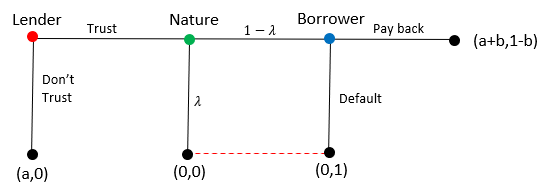
\includegraphics[scale=.8]{figure1.png}
\end{center}
We can find the subgame perfect equilibrium via backward induction. The borrower is the last player to move (if they get the chance to move), and they have the choice between defaulting and getting a payoff of 1, or paying the lender back to get a payoff of ${1-b}$. Their optimal move is to default, leading to a payoff of 0 for the lender. The lender, then, is faced with the decision to trust the borrower, and get a payoff of zero\footnote{Since the borrower defaults regardless of whether the project is a success, the lender faces this payoff regardless of $\lambda$.}, or not trust the borrower and get a payoff of $a>0$. Thus, the SPE is (don't trust, default).

%%%________________________________________________________________%%%

\subsection*{Question 3}

\begin{enumerate}[(a)]
	\item If $n=1$, the subgame perfect equilbrium is for the player who wins the coin toss to offer 0 to the other player, keeping 1 for themselves, and for the toss-losing player to accept the offer. Since the offering player is chosen by a fair coin, each player's expected value of this game is ${\frac{1}{2}(\delta^00) + \frac{1}{2}(\delta^01) = \frac{1}{2}}$. 
	
	\item If the game makes it to $t=1$, then the winner of the coin toss will offer the other player 0, resulting in a payoff of $\delta$ for the coin toss winner and 0 for the other player. At $t=0$, both players understand this, so the player who loses the first-round coin toss will reject any offer less than their expected payoff in the second round, ${\frac{1}{2}\delta}$. The player who wins the first-round toss is willing to make any offer that would ensure a higher payoff than their expected payoff given another coin toss (which is equal to the toss-losing player's expected payoff). Since ${1-\frac{1}{2}\delta>\frac{1}{2}\delta}$, the winner of the first-round toss is willing to offer the loser of the toss the lowest amount that they would accept, ${\frac{1}{2}\delta}$. Thus, the SPE is for the winner of the first coin toss to offer $\frac{1}{2}\delta$, and for the losing player to accept.
	
	The expected value of this game to each player is
	\[
		\frac{1}{2}\left(1-\frac{1}{2}\delta\right)+\frac{1}{2}\left(\frac{1}{2}\delta\right) = \frac{1}{2} - \frac{1}{4}\delta + \frac{1}{4}\delta = \frac{1}{2}
	\]
	
	\item Suppose $n\geq 3$ and the game makes it to ${t=n-2}$. The winner of the final toss will offer their opponent 0 and earn a payoff of $\delta^{n-1}$. Then, in ${t=n-2}$, the loser of the coin toss will accept any offer at or above $\frac{1}{2}\delta^{n-1}$, so the game would end with the winner offering ${\frac{1}{2}\delta^{n-1}}$ and winning ${\delta^{n-2}\left(1-\frac{1}{2}\delta^{n-1}\right)}$. Then, in  ${t=n-3}$, each player's expected payoff is $\frac{1}{2}\delta^{n-2}$, once again allowing the winner of the prior-round coin toss to make an acceptable offer to that round's toss loser. This reamins true for every ${t>0}$, resulting in an SPE where the winner of the first coin toss offers $\frac{1}{2}\delta$, which is accepted by the loser of the first coin toss.
	
	Thus, the value of this game to each player, regardless of $n$, is $\frac{1}{2}$.
	
\end{enumerate}

%%%________________________________________________________________%%%
\pagebreak
\subsection*{Question 4}
Following the firms' price and location decisions, each consumer faces the following optimization problem:
\[
	\usmin{i}\left\{p_i + c\left(w-x_i\right)^2\right\}
\]
Thus, assuming that each coffee lover buys the same amount of coffee, firm $i$ seeks to maximize per-cup expected profits, $\pi_k$ from each consumer. Assuming the firm faces zero costs without loss of generality,\footnote{This assumption results in the same decision rule for each firm in all cases except for those when variable costs are nonzero and the firm faces a lower bound on its price at the shutdown price.}
\[
	\pi_k = \begin{cases} 	p_i, & p_i - p_j < c\left[(w_k-x_j)^2 - (w_k-x_i)^2\right] \\ \frac{1}{2}p_i, & p_i - p_j = c\left[(w_k-x_j)^2 - (w_k-x_i)^2\right] \\ 
							0, & p_i - p_j > c\left[(w_k-x_j)^2 - (w_k-x_i)^2\right]	\end{cases}
\]
Where ${j\neq i}$ is the rival coffee shop. Solving this inequality for $w_k$ allows us to find the cutoff value, $w^*$, for which, holding prices constant, a consumer will patronize coffee shop $i$:
\begin{align*}
	p_i - p_j &\leq c\left[(w^*-x_j)^2 - (w^*-x_i)^2\right] = c\left[2w^*(y_i-y_j) + y_j^2-y_i^2\right]	\\
	2w^*(y_i-y_j) &\geq \frac{1}{c}(p_i-p_j) - y_j^2 + y_i^2 	\\
	w^* &\leq 	\begin{cases} 	\frac{p_i - p_j}{2(y_i - y_j)} + \frac{1}{2}(y_i + y_j), & y_i<y_j \\
								\frac{p_i - p_j}{2(y_j - y_i)} - \frac{1}{2}(y_i + y_j), & y_i>y_j
				\end{cases}
\end{align*}
If the rival coffee shops co-locate, then they will compete on price alone. Thus, expected profits depend on both relative location and relative prices, each with three possibiliies. Since we know the distribution of $w_k$, we can derive firm $i$'s total expected profits $\pi$, given $(p_1,p_2)$ and $(x_1,x_2)$, which is best summarized in a matrix:\footnote{The values in the matrix for all cases except ${y_i=y_j}$ were determined by integrating over the distribution of $w$. For example, expected profit for the ${y_i<y_j}$ cases were calculated with: $$ \int_0^{w^*}p_idF(w) = p_i\left(\frac{p_i - p_j}{2(y_i - y_j)} + \frac{1}{2}(y_i + y_j)\right) $$}
\[
	[]
\]
Firm $i$'s best response function for the pricing decision, then, is 
\[
	[]
\]


%%%________________________________________________________________%%%


\end{document}




































